\documentclass[12pt, a4paper, lithuanian]{article}
\usepackage[utf8x]{inputenc}
\def\LTfontencoding{L7x}
\PrerenderUnicode{ąčęėįšųūž}
\usepackage[\LTfontencoding]{fontenc}
\usepackage[lithuanian]{babel}
\usepackage{VUMIF}
\usepackage{cite}
\usepackage{amsmath}
\usepackage{bm}
\usepackage{amsfonts}
\usepackage{float}
\usepackage{graphicx}
\usepackage{color}
\usepackage{listings}
\usepackage{wrapfig}
\usepackage{algpseudocode}
\usepackage{algorithm}
\usepackage{algorithmicx}
\usepackage{caption}
\usepackage{subfig}

\makeatletter
\renewcommand{\ALG@name}{Algoritmas}
\DeclareCaptionLabelFormat{numberfirst}{#2 \ALG@name}
\captionsetup[algorithm]{labelformat=numberfirst} 
\makeatother

\DeclareMathOperator*{\argmin}{arg\,min}
\DeclareMathOperator*{\argmax}{arg\,max}

% Titulinio aprašas
\vumifdept{Programų sistemų katedra}
\vumifpaper{Magistro baigiamasis darbas}
\title{Klaidų kainoms jautrūs klasifikavimo algoritmai}
\def\titleineng{Cost-sensitive classification algorithms}
\def\statusas{% Kai kurioms katedroms reikia nurodyti  
    2 kurso 1 grupės studentas \\
}
%% Jeigu 1 autorius:
\author{
   Vardaitis Pavardaitis 
}
%% Jeigu 2 autoriai:
%\def\authone{
%    Vardaitis Pavardaitis
%}
% \def\authtwo{
%    Vardaitė Pavardaitė
% }

\supervisor{prof. hab. dr. Vardenis Pavardenis}
\reviewer{dr. Vardonis Pavardonis}
\date{Vilnius \\ 2014}

\begin{document}
\sloppy
\maketitle

\vumifsectionnonumnocontent{Santrauka}

Praktiniuose taikymuose, kaip kad medicinos diagnostikoje ir veidų atpažinime, pripažintas santykinis klasifikavimo klaidų kainų, priklausančių nuo tikrosios ir priskirtosios klasių, skirtumas. Šis darbas apima klaidų kainoms jautraus hibridinio klasifikatoriaus, sudaryto iš sprendimo medžio ir daugiasluoksnio perceptrono, kūrimą ir analizę. Hibridiniam klasifikatoriui konstruoti buvo realizuoti kainoms jautrių \emph{C4.5} sprendimo medžių variantai bei klaidų kainoms jautrus daugiasluoksnis perceptronas, jiems kombinuoti panaudota \emph{Banerjee} metodika. Atlikti eksperimentai su realaus pasaulio ir sintetiniais duomenimis leidžia teigti, kad hibridinis klasifikatorius gali būti naudingas, t. y. sumažinti jį inicializavusio sprendimo medžio klasifikavimo kainą ir pasiekti šį rezultatą greičiau nei atsitiktiniais svoriais inicializuotas daugiasluoksnis perceptronas.

\bigskip
Raktiniai žodžiai: nesubalansuoti duomenys, jautrus kainoms, klasifikavimas, dirbtiniai neuroniniai tinklai, sprendimų medis, hibridinis, daugiasluoknis perceptronas.


\vumifsectionnonumnocontent{Summary}

In practical applications including medical diagnosis and face detection it has been admitted that classification errors might differ in relative cost depending on the real and predicted classes. The work comprises implementation and analysis of a cost-sensitive hybrid classifier, consisting of a decision tree and a multi-layer perceptron. The hybrid classifier was constructed using several varieties of a cost-sensitive \emph{C4.5} decision tree and a cost-sensitive multi-layer perceptron, which were combined using the \emph{Banerjee} method. Conducted experiments with real world and synthetic data allow to conclude that the hybrid method might be useful, namely, decrease the misclassification error cost of the initializing tree and achieve this result faster than a randomly initialized multi layer perceptron.

\bigskip
Keywords: imbalanced dataset, cost-sensitive, classification, artificial neural network, decision tree, hybrid, multilayer perceptron.


\tableofcontents

\vumifsectionnonum{Terminai}
\begin{enumerate}
\item ANT - klasikinis atgalinio perdavimo neuroninis tinklas (angl.
back-propagation neural network)
\item DNT - dirbtinis neuroninis tinklas (angl. artificial neural network)
\item DSP - daugiasluoksnis perceptronas (angl. multilayer perceptron)
\item ...
\end{enumerate}


\vumifsectionnonum{Įvadas}
Klasifikavimo uždavinį naudojant induktyvaus pobūdžio mokymąsi plačiai mėginta spręsti orientuojantis į klasifikavimo klaidų skaičiaus minimizavimą. Panaudojant aibę mokymosi duomenų - vektorių, kuriems įvardyta priklausomybė tam tikrai klasei, - konstruojamas algoritmas, besistengiantis kuo didesnį skaičių elementų priskirti teisingai klasei.

...

Keliama tokia \textbf{hipotezė}:

\emph{Įmanoma panaudoti pavienį sprendimo medį, kurio apmokymas greitas, tačiau jautrumas kainoms silpnas, inicializuoti tinklui, kurio architektūra ir parametrai nežinomi, be to, apmokymas lėtas, tačiau jautrumas kainoms geras, kad būtų gautas greitai apmokomas gero jautrumo kainoms klasifikatorius.} 

...


\section{Klasifikavimo uždavinys}

% A review of crucial concepts in the problem of classification. 
Klasifikavimo problema - kaip pagal turimus duomenis\footnote{Pusjuodės
didžiosios raidės žymi matricas.} $\bm{D}$, kurie susideda iš $n$ duomenų taškų
(vektorių\footnote{Pusjuodės mažosios raidės žymi vektorius.}) $\bm{x}_i \in
\mathbb{R}^p$, $i = 1, ..., n$, bei žinomas jų klases $class(\bm{x_i}) \in
\{1, 2, ..., m\}$, $i = 1, ..., n$, sudaryti metodą, kuris galėtų nustatyti vektoriaus
$\bm{x'} \in \mathbb{R}^p$ klasę.

Nagrinėjant realaus pasaulio duomenis iškyla dvi problemos \cite{RountreePhDThesis}:

...


\section{Dirbtinių neuroninių tinklų apžvalga}
\label{sec:Dirbtiniu neuroniniu tinklu apzvalga}

\subsection{Bendrieji dirbtinių neuroninių tinklų principai}
\subsubsection{Perceptronas}
\label{sec:Perceptronas}
Perceptronas\footnote{Perceptronu vadinsime McCulloch-Pitts neuroną su
sigmoidine aktyvavimo funkcija.} yra iteraciškai apmokomas tiesinis
klasifikatorius. % Perceptrono atliekamų veiksmų seką galime aprašyti taip:
Įvedami žymėjimai:
duomenų vektorių $\bm{x} = (x_1, x_2, ..., x_p)$ praplečiame vienetu, $\bm{z} =
(1, x_1, x_2, ..., x_p)$, perceptrono įėjimų svorių vektorių $\bm{w} = (w_1,
w_2, ..., w_p)$ praplečiame $w_0$, $\bm{v} = (w_0, w_1, w_2, ..., w_p)$.
Naudosime sigmoidinę glodninimo funkciją:
\begin{equation} \label{eq:sigmoid}
f(x) = {1 \over 1 + e^{-x}} \;.
\end{equation}

Tada $i$-tajam duomenų vektoriui perceptrono išėjimas apskaičiuojamas taip:
\begin{equation} \label{eq:perceptron output}
o_i = f(\bm{x}_i \bm{w}^T + w_0) = f(\bm{z}_i \bm{v}^T) \;.
\end{equation}

...


\section{Sprendimo medžių apžvalga}
\label{sec:Sprendimo medziu apzvalga}

\subsection{Bendrieji sprendimo medžių principai}

Sprendimo medžiu vadinamas medžio pavidalo klasifikatorius, priskiriantis klasėms daugiamačius vektorius, kurių požymiai gali būti tiek kategoriniai, tiek tolydieji kintamieji. %[TODO: savybės: privalumai, trūkumai]

Medį sudaro arba lapas, pažymėtas klasės etikete, arba struktūra, apimanti su dviem ar daugiau pomedžių sujungtą sprendimo priėmimo mazgą \cite{DBLP:dblp_journals/csur/Quinlan96}. Pastarosios rūšies mazgai apibrėžiami testo pavidalu, o jų pomedžiai atitinka visas įmanomas šio testo baigtis (pvz., žr. \ref{fig:DT}).
\begin{figure}[H]
  \centering
    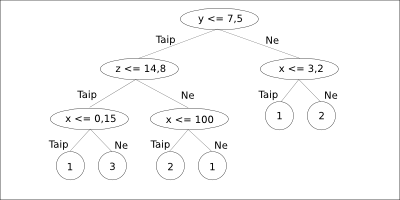
\includegraphics{skyriai/paveiksliukai/sm_pvz}
  \caption{Sprendimo medžio pavyzdys\label{fig:DT}}
\end{figure}

...


\section{Algoritmų realizacija}
\subsection{Dirbtinių neuroninių tinklų realizacija}
\label{sec:Dirbtinių neuroninių tinklų realizacija}

Norint geriau susipažinti su klasifikavimo klaidų kainų įvedimo metodais bei jų
savybėmis, prieš kuriant SM ir DNT kombinuojantį klasifikatorių, buvo nuspręsta atskirai
išsinagrinėti kainų įvedimo metodus į SM ir DNT klasifikatorius. Atlikus kainų
įvedimo į DNT metodų analizę (žr. ~\ref{sec:Perceptronas} skyrių) paaiškėjo,
kad geriausias duomenų subalansavimo metodas yra (\ref{eq:sigmoid}), o
praktikoje nusistovėjęs kainų įvedimo į DNT metodas yra (\ref{eq:perceptron output}),
kuris ir realiuotas šiame darbe.

...

\subsection{Sprendimo medžių realizacija}
\subsubsection{Medžio konstravimas MetaCost algoritmu}\label{sec:Medžio konstravimas MetaCost algoritmu}

Šiame darbe realizuoto MetaCost algoritmo pseudokodas pateiktas \ref{alg:MetaCost pseudokodas} algoritme. Įeities duomenys yra: $S$ - mokymo duomenys, $L$ - klasifikavimo algoritmas, $C$ - kainų matrica, $m$ - mokymo duomenų vektorių atsitiktinių rinkinių skaičius, $n$ - vektorių skaičius atsitiktiniame mokymo duomenų poaibyje.

\begin{algorithm}
\caption{MetaCost algoritmo pseudokodas.}
\begin{algorithmic}[1]
    \Procedure{MetaCost}{$S, L, C, m, n$}
        \For{$i\gets 1, n$}
            \State $S_i$ yra n ilgio vektorių rinkinys iš $S$ aibės
            \State $M_i$ yra klasifikatorius, gautas $L$ algoritmą apmokius su $S_i$
        \EndFor
        \State $S'\gets \emptyset$
        \ForAll{$x \in S$}
            \ForAll{$j \in classes$}
                \State $P(j|x) \gets {1 \over  \sum_i 1} \sum_i P(j|x, M_i)$, kur 
                \State $\forall i P(j|x, M_i) = \left\{
                    \begin{array}{lr} 
                        1 & : \text{jei $M_i$ prognozuoja klasę j} \\ 0 & : \text{priešingu atveju} \\
                    \end{array} \right. $ 
            \EndFor
            \State $x$ nauja klasė $\gets \underset{i}{\argmin} \sum_j P(j|x) C(i,j)$
            \State $S'\gets S' \cup x$
        \EndFor
        \State \textbf{return} Klasifikatorius, gautas apmokius algoritmą L su kainų atžvilgiu palankiausiai perklasifikuotais duomenimis $S'$ 
    \EndProcedure{}
\end{algorithmic}
\label{alg:MetaCost pseudokodas} 
\end{algorithm}

...


\section{Hibridinių klasifikatorių veikimo eksperimentinis tyrimas}

\subsection{Bendrieji eksperimentų nustatymai}

Eksperimentais šiame skyrelyje siekiama nustatyti, ar apskritai yra prasminga kurti kainoms jautrų hibridinį klasifikatorių, panaudojant SM ir DNT hibridizacijos metodiką \cite{Banerjee1997} ir įvedant jautrumą kainoms kiekvienoje klasifikatoriaus dalyje nepriklausomai. Kad būtų prasminga, reikėtų parodyti, kad hibridinis klasifikatorius sugeba pasiekti mažesnę klasifikavimo kainą su testiniais duomenimis nei jį inicializavęs sprendimo medis per mažiau iteracijų nei tokios pat architektūros, tačiau atsitiktiniais svoriais inicializuotas DSP.

...

\begin{table}[h!]
  \begin{center}
    \begin{tabular}{|c|p{4.5cm}|p{5cm}|p{3.5cm}|}
      \hline
      & \multicolumn{1}{|c|}{Pavadinimas} & {Inicializuojantis medis} & {Kainoms jautrus algoritmo aspektas} \\
      \hline
      1. & \emph{Hybrid\_C4.5} & C4.5 medis & DSP \\
      2. & \emph{Hybrid\_Laplace} & C4.5 medis, Laplace genėjimas & Genėjimas, DSP \\
      3. & \emph{Hybrid\_MetaCost} & MetaCost medis, naudojantis C4.5 medį kaip bazinį klasifikatorių & MetaCost, DSP \\
      4. & \emph{Hybrid\_Mod\_prob} & C4.5 medis, pakeitus apriorines klasių tikimybes ir lapų klases pagal kainų matricą & Tikimybių modifikacija ir lapų pernumeravimas, DSP \\
      5. & \emph{Hybrid\_Mod\_prob\_err} & C4.5 medis, pakeitus apriorines klasių tikimybes pagal kainų matricą, klaidomis grįstas genėjimas & Tikimybių modifikacija, DSP\\
      6. & \emph{Hybrid\_Mod\_prob\_lap} & C4.5 medis, pakeitus apriorines klasių tikimybes pagal kainų matricą, Laplaso genėjimas & Tikimybių modifikacija, genėjimas, DSP \\
      7. & \emph{Hybrid\_C5.0} & C5.0 medis & C5.0 medis, DSP \\
      8. & \emph{Banerjee} & C4.5 medis & Kainoms nejautrus \\
      \hline
    \end{tabular}
  \end{center}
  \caption{Lyginami hibridiniai klasifikatoriai.}\label{tab:implemented classifiers}
\end{table}

...


\vumifsectionnonum{Išvados}

Šiame darbe realizuota:
\begin{enumerate}
\item Sukurta bazinė C4.5 algoritmo realizacija ir keli jautrumo kainoms joje užtikrinimo metodai: gaubiamasis MetaCost algoritmas, pakeistosios klasių tikimybės, Laplace genėjimas. 
\end{enumerate}

...

Atlikus eksperimentus su sintetiniais ir realaus pasaulio duomenimis, gautos tokios išvados:
\begin{enumerate}
\item Parodyta, kad hibridinis kainoms jautrus klasifikatorius, paremtas \cite{Banerjee:1997:INN:267553.267554} hibridizacijos metodika ir jautrumo kainoms įvedimu į sprendimo medį bei daugiasluoksnį perceptroną atskirai, gali sumažinti inicializavusio sprendimo medžio klasifikavimo klaidų kainą su testiniais duomenimis. Taip pat parodyta, kad hibridas pasiekia geriausios kainos iteraciją greičiau nei analogiškos architektūros, tačiau atsitiktinių pradinių svorių daugiasluoksnis perceptronas.
\end{enumerate}

...


\bibliography{skyriai/bibliografija}

\appendix
\section{Papildomų eksperimentų rezultatų lentelės}

\begin{table}[h]
\caption{Rezultatai su \emph{Tae} duomenimis. \emph{Banerjee} ir hibridiniai klasifikatoriai, taip pat medžiai ir jų hibridai lyginami pagal klaidų kainą, o DSP ir hibridai - pagal mokymosi iteracijų skaičių.}
{\begin{tabular}{@{}lllllllll@{}} \hline
             & $\bar{x}$ & $\sigma^{2}$& \multicolumn{3}{|c|}{$a > b$}  &  \multicolumn{3}{|c}{$a < b$} \\
\hline
Algoritmas &            &            & & p/2 & T        & & p/2 & T \\
\hline
$a)$ Banerjee & 1.6335 & 0.5584 & N & 0.0000 & -5.1173 & T & 0.0000 & 5.1173 \\
$b)$ Hybrid\_C50 & 1.7395 & 0.5647 &  &  &  &  &  & \\
\hline
$a)$ C50 & 1.7490 & 0.5819 & N & 0.3047 & 0.5109 & N & 0.3047 & -0.5109 \\
$b)$ Hybrid\_C50 & 1.7395 & 0.5647 &  &  &  &  &  & \\
\hline
$a)$ DSP & 82.1200 & 244.7042 & T & 0.0112 & 2.2845 & N & 0.0112 & -2.2845 \\
$b)$ Hybrid\_C50 & 63.2800 & 202.4601 &  &  &  &  &  & \\
\hline
\hline
$a)$ Banerjee & 1.6335 & 0.5584 & T & 0.0000 & 35.0309 & N & 0.0000 & -35.0309 \\
$b)$ Hybrid\_Laplace & 0.7147 & 0.1800 &  &  &  &  &  & \\
\hline
$a)$ Laplace & 0.6894 & 0.1159 & N & 0.0045 & -2.6250 & T & 0.0045 & 2.6250 \\
$b)$ Hybrid\_Laplace & 0.7147 & 0.1800 &  &  &  &  &  & \\
\hline
$a)$ DSP & 82.1200 & 244.7042 & T & 0.0000 & 12.4643 & N & 0.0000 & -12.4643 \\
$b)$ Hybrid\_Laplace & 0.6100 & 1.3107 &  &  &  &  &  & \\
\end{tabular}}
\label{tab:tae dataset ttests}
\end{table}



\end{document}
